\section{Proposed Method}\label{sec:approach}
% \begin{figure*}[t]
% \centering
%   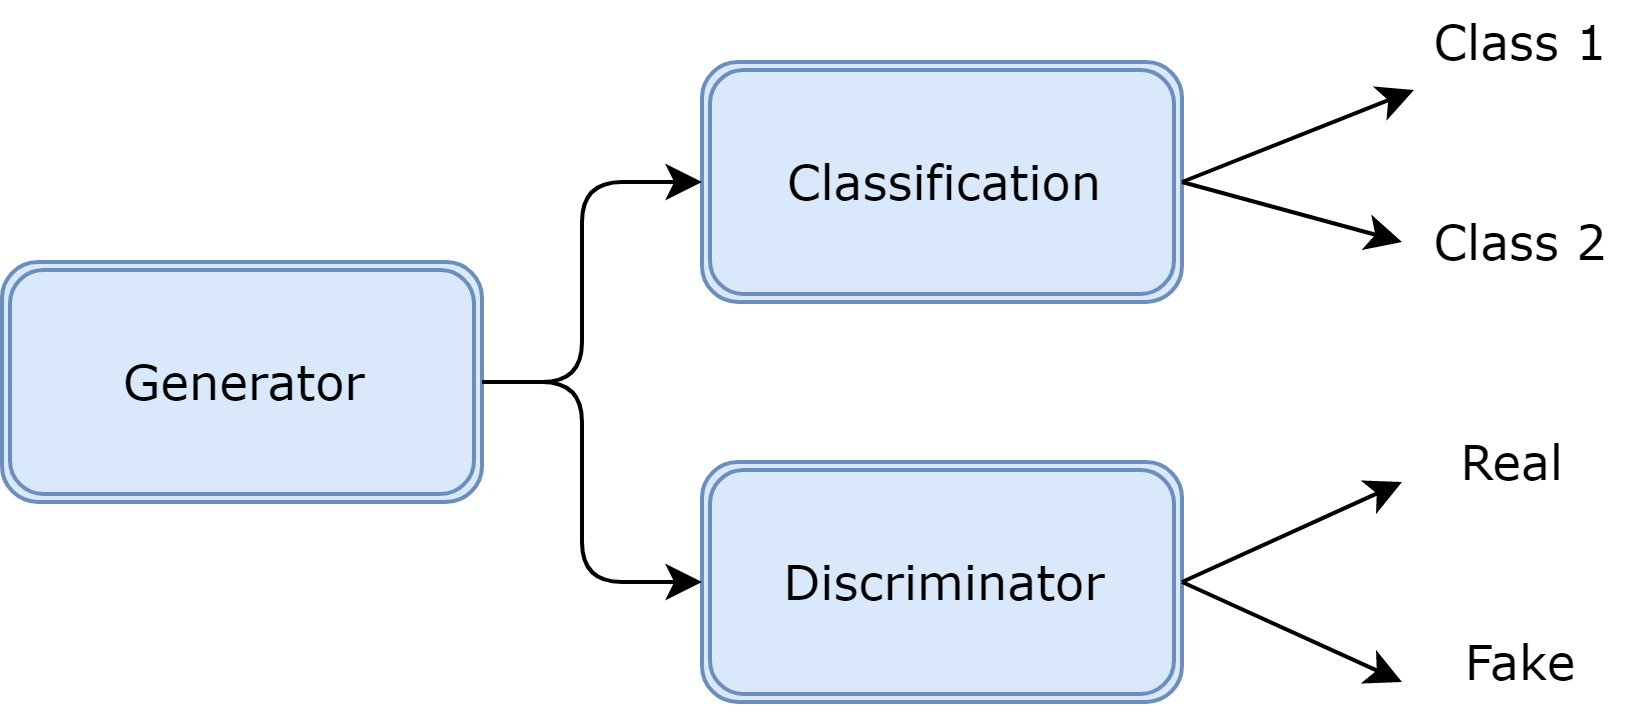
\includegraphics[width=0.5\textwidth]{gcdArch.jpg}
%   \caption{GAN Architecture}
%   \label{fig:gcdarch}
%   \vspace{20pt}%
% \end{figure*}

\begin{figure*}[t]
\centering
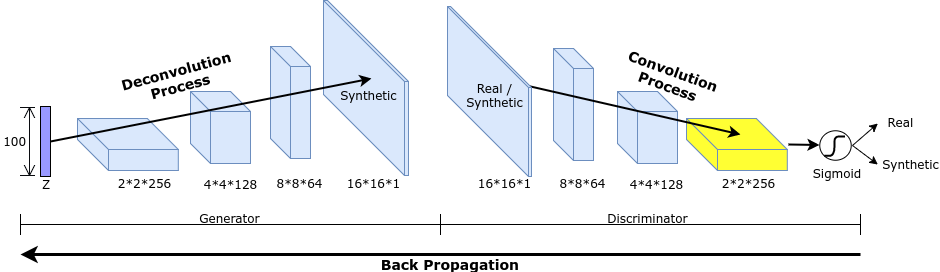
\includegraphics[width=0.7\textwidth]{GAN-Dicriminator.png}
\vspace{-1em}
\caption{Our table-GAN architecture. The classifier is omitted because of space limitations, and it has the same neural network architecture as the discriminator. The generator (resp. discriminator) performs a series of deconvolution (resp. convolution) operations to generate (resp. classify) a record. The final loss after the sigmoid activation can be back-propagated to the generator. The dimensions of the latent vector input $z$ and intermediate tensors should be configured considering the number of attributes (e.g., $16 \times 16=196$ attributes in this figure).}
  \label{fig:gdlayers}
\end{figure*}

We introduce the proposed table-GAN that, given a table to synthesize and several parameters to control the privacy level, generates a synthetic table that is statistically similar to the original table.


\subsection{Neural Network Architecture}
The deep convolutional GAN (DCGAN) is one of the most influential works for GANs. Many meaningful ideas have been proposed to design the neural network architecture of the generator ($G$) and the discriminator ($D$), as follows: (1) replacing spatial pooling functions with strided convolutions, (2) eliminating fully connected hidden layers, and (3) using batch normalization~\cite{conf/icml/IoffeS15}, ReLU for the generator~\cite{icml2010_NairH10}, and LeakyReLU~\cite{maas2013rectifier} for the discriminator.

Our model also adopts the DCGAN architecture but has an additional neural network called \textit{classifier} ($C$), as follows:
\begin{itemize}
\item A generator neural network $G$ to produce synthetic records that have the same distribution as that of real records;
\item A discriminator neural network $D$ to distinguish between real and synthetic records;
\item A classifier neural network $C$ to predict synthetic records' labels. We found that adding $C$ helps maintain the consistency of values in the generated records. For instance, a record with gender = ``Male'' and disease = ``Uterine Cancer''  can be prevented; the classifier learns about the consistency from the original table.
\end{itemize}

We describe neural network architectures in more detail in the following.
% GANs basically contain two competing neural networks. One of these networks generates samples and the other one discriminates the real samples from the generated ones. These two networks are trained simultaneously until they converge to a point that the generated samples can not be distinguished from real ones with high confidence.  
% functions....

\subsubsection{Discriminator}
The discriminator network $D$ is a neural network trained to classify the generated records as \textit{synthetic} and the records in the original table as \textit{real}. 
% The inputs to this network are training data form the original dataset and the generated samples from the generator component. 
Precisely, $D$ is a convolutional neural network (CNN) that contains multiple layers. In each layer, a list of learnable filters (e.g., 3$\times$3 matrices) are applied to the entire input matrix (i.e., convolution operations). Recall that records are converted into square matrices in our method. Thus, the layer output size is proportional to the number of filters in each layer.

The output of a layer is the input to the next layer, as shown in Figure~\ref{fig:gdlayers}. The dimension of intermediate tensors keeps decreasing and the depth continues increasing until the last sigmoid activation layer that generates the probability of being real or synthetic. There are other intermediate layers (omitted in Figure~\ref{fig:gdlayers}) that affect the functionality of the network, such as batch normalization or LeakyReLU~\cite{radford_dcgan_2015}.

% Each filter has different parameters (weights and biases) to be learned and these learnable parameters are tuned during the back-propagation mechanism\cite{}. Back-propagation is an iterative learning mechanism which starts from the last layer and backwards the initial layers to tune the parameters of the each layer in order to reach the best prediction results out of the neural network. The learning process needs a metric to measure the efficiency of the learning steps. Loss or cost functions are used to measure the differences between the current outcome of the neural network and the desired results. The goal of the training mechanisms is to find the best values for parameters of the neurons by minimizing the loss functions. The learning algorithms achieve these goal by using the descending gradients(vector of partial derivatives) of the loss functions to calculate the new values for the parameters in each learning iteration. We utilizes the standard learning technique used in the neural networks called Stochastic Gradient Descent(SGD) which uses a small randomly selected portion of the training data to calculate the gradients. We also use the Adam algorithm \cite{} as the optimizer algorithm for the SGD technique.\\

The input to the first layer is a $d \times d$ matrix that represents one real or synthetic record. The discriminator is trained to predict 1 for real records and 0 for synthetic records after the last sigmoid layer.

If the number of attributes in the original table is less than the input size, then each record is padded with zeros and reshaped into a square matrix. Our model is configurable and able to learn from a table with many attributes (e.g., $16 \times 16 = 256$ attributes in a single table and some GANs supports images that are as large as $1024 \times 2014$~\cite{2017arXiv171010196K}).
% To minimize the side-effects of the zero-padding, we duplicate records multiple times and minimize the number of padded zeros.   
% The feature of the input samples ( form both training data and generated samples) will be extracted through the convolutional layers and the final layer uses the activation functions to generate the probability of being fake or real. 

% D Shape image : (64, 8, 8, 1)
% D Shape h0: (64, 4, 4, 3)
% D Shape h1: (64, 2, 2, 66)
% D Shape h3: (64, 1)

% G shape z : (64, 100)
% G Shape h0: (64, 1, 1, 256)
% G Shape h2: (64, 2, 2, 128)
% G Shape h3: (64, 4, 4, 64)
% G: Shape h4: (64, 8, 8, 1)

\subsubsection{Generator}
The generator $G$ is also a neural network that consists of multiple de-convolutional layers. As shown in Figure~\ref{fig:gdlayers}, $G$ performs a process that is opposite to that of the discriminator. Its input is a latent vector $z$ that is uniformly sampled from the unit hypercube space\footnote{A high-dimensional space where each dimension is confined to the range of [-1,1]}. Multiple de-convolutional layers convert the input $z$ to a 2-dimensional matrix corresponding to a record in the synthetic table.

The generator can be trained by the discriminator's prediction result (in fact, this is one of the multiple ways we propose to train the generator in our table-GAN). Its goal is to deceive the discriminator. This training process can be very efficiently implemented by back-propagation.
% In fact, the generator learns the features of the training dataset in respect to its attributes(columns) in a MinMax game mechanism.  In this mechanism the generator network's parameters are repeatedly (learning process contains many iterations) tunned in such way that the generated samples can fool the discriminator to classify them as real ones with the lowest possible error rate in each iteration. The parameter tuning mechanism is based on the traditional back-propagation techniques used in neural networks. We use the Stochastic Gradient Descent(SGD) as the learning optimization technique. More  here ... //

% The training algorithms aims to train G to be a good estimator of training data(x).
% The convolutional layers in the generator component

% by propagating the errors to  rate to the  learning mechanism is is done using the back propagation mechanism and the learning optimization techniques such as SGD.
% At the end of training the generator is in a state that can generate desired samples similar to the original dataset.
% Is it correct this way? More details about the convolutional layers, and their dimensions?

\subsubsection{Classifier}\label{sec:class}
The classifier network $C$ has the same neural network architecture as the discriminator. However, it is trained by ground-truth labels in the original table. In Table~\ref{T:example}, for instance, the diabetes attribute contains ground-truth labels. Therefore, the classifier is trained to learn about the correlation between the cholesterol and diabetes attributes from the table. Given a synthetic record, it can teach the generator whether the record is semantically correct. For example, (cholesterol=50, diabetes=1) is not a correct record because cholesterol=50 is too low to be diagnosed as diabetes. If such records are synthesized by the generator, the classifier can effectively correct the generator.

In fact, the discriminator itself can learn about the semantic integrity to some degree. Semantically incorrect generations are likely not to be classified as real by the discriminator. However, it does not mainly consider about the semantic integrity and we found some incorrect generation examples without the classifier.


\subsection{Loss Functions}
The loss function contains the philosophy for training neural networks. In general, neural networks are trained by minimizing a loss function, and ill-designed loss functions deteriorate the training process and lead to malfunctioning neural networks. Therefore, the design of loss functions to train the three proposed neural networks is key for successful table syntheses. We adopt one loss function from DCGAN and design two more loss functions, as follows:

\begin{enumerate}
\item The \textit{original loss} is adopted from DCGAN and was already shown in Equation~\ref{eq:gan}.
\item The \textit{information loss} is defined as the discrepancy between two statistics of synthetic and real records.
\item The \textit{classification loss} is defined as the discrepancy between the predicted label by the classifier and the synthesized label.
\end{enumerate}

% Loss functions determines 

% In the remaining of the paper we use the following notation
% and terminology:
% X - the clean training data from the dataset.
% y : the label for training data
% J(X, y): the cost function to be minimized for training.

\textbf{The discriminator is trained with the original DCGAN loss, and the classifier is trained with the classification loss. The generator is trained with all three loss functions because it is the most important neural network in our method.} In this subsection, we introduce the individual loss functions.

\subsubsection{Original Loss}
The original DCGAN loss function is shown in Equation~\ref{eq:gan}. The discriminator is trained to maximize it, and the generator is trained to minimize it. It represents the training philosophy of GANs (i.e., while the generator attempts to deceive the discriminator, it can significantly improve its synthesis capability). See~\cite{goodfellow2014generative,radford_dcgan_2015} for more detailed descriptions of the original loss. There are also some variations of the original loss~\cite{2017arXiv170104862A}, but the most widely used one is still the one we already introduced.

The exact loss function to train the discriminator can be written as follows:
\begin{equation}\label{eq:origD}\begin{aligned}
\Loss_{orig}^{D} = & -\mathbb{E}[\log D(x)]_{x \sim p_{data}(x)} \\
  & - \mathbb{E}[\log (1-D(G(z)))]_{z \sim p(z)},
\end{aligned}\end{equation}
and the generator can be written as follows:
\begin{equation}\label{eq:origG}\begin{aligned}
\Loss_{orig}^{G} = \mathbb{E}[\log (1-D(G(z)))]_{z \sim p(z)}.
\end{aligned}\end{equation}

Note that we added negative signs in $\Loss_{orig}^{D}$ to convert the maximization of Equation~\ref{eq:gan} to the minimization. Deep learning algorithms typically prefer to minimize losses. There are multiple different ways to implement the loss in program codes but it is usually calculated using cross entropy\footnote{One example is the DCGAN implementation in \url{https://github.com/carpedm20/DCGAN-tensorflow/blob/251aa440013afb86ddfefef8ddce3629be7972ac/model.py#L124}.}.

\subsubsection{Information Loss}
To define the information loss, we extract features immediately before the sigmoid activation of the discriminator network (i.e., the flattened tensor marked in yellow in Figure~\ref{fig:gdlayers}). From these features, the discriminator decides whether the inputs are real or synthetic. Thus, \textbf{it is reasonable to say that the extracted features contain key characteristics of the input samples}. In general, extracted features become very high-dimensional vectors after flattening. We use bold font $\f$ to denote these vectors.

The simplest form of information loss is as follows:
\begin{equation}\label{eq:mean}\begin{aligned}
\Loss_{mean} =  & \| \mathbb{E}[\f_x]_{x \sim p_{data}(x)} - \mathbb{E}[\f_{G(z)}]_{z \sim p(z)}\|_2,
\end{aligned}\end{equation}
where $\f$ stands for features (i.e., high-dimensional vectors) extracted from the last layer of the discriminator and $\mathbb{E}[\f]$ means the average feature (i.e., the centroid of the vectors) of all records in the dataset. Note that we use the L-2 norm (Euclidean norm) to measure the discrepancy between two mean features (vectors).

Thus, $\Loss_{mean}$ is to compare the first-order statistics (i.e., mean) of the features of real and synthetic records. We also use the second-order statistics (i.e., standard deviation) as follows:
\begin{equation}\label{eq:std}\begin{aligned}
\Loss_{sd} =  & \| \mathbb{SD}[\f_x]_{x \sim p_{data}(x)} - \mathbb{SD}[\f_{G(z)}]_{z \sim p(z)}\|_2,
\end{aligned}\end{equation}
where $\mathbb{SD}[\cdot]$ represents the standard deviation of features.

$\Loss_{mean}=0$ and $\Loss_{sd}=0$ mean that real and synthetic records  have the statistically same features from the perspective of the discriminator (recall that the extracted features are from the last layer of the discriminator). This further implies that the discriminator may not be able to distinguish them.

\textbf{The quality of the synthesis process should be controllable}. With unreliable partners, you may not want to share a synthetic table that is very similar to the original table. You may want to intentionally generate a low-quality table in that case. For this purpose, we design the following loss to train the generator based on the hinge-loss that does not incur any loss until a predetermined quality degradation threshold:
\begin{equation}\begin{aligned}
\Loss_{info}^{G} =  & \max(0, \Loss_{mean}-\delta_{mean}) + \max(0, \Loss_{sd}-\delta_{sd}).
\end{aligned}\end{equation}

The information loss $\Loss_{info}^G$ provides zero loss as long as $\Loss_{mean}$ (resp. $\Loss_{sd}$) is smaller than a threshold $\delta_{mean}$ (resp. $\delta_{sd}$). Thus, $\delta_{mean}$ and $\delta_{sd}$ are two parameters for controlling the level of privacy. If these parameters are small, then the privacy level will be lower, and the synthetic table will be similar to the original table.

\subsubsection{Classification Loss}
We found that  values occasionally do not match with labels in synthetic records, as stated in Section~\ref{sec:class}. To avoid this situation, we design an additional loss function called \textit{classification loss}, as follows:
\begin{equation}\label{eq:class}\begin{aligned}
\Loss_{class}^{C} =  & \mathbb{E}[|\ell(x)-C(remove(x))|]_{x \sim p_{data}(x)},
\end{aligned}\end{equation}
\begin{equation}\begin{aligned}
\Loss_{class}^{G} = &\mathbb{E}[|\ell(G(z))-C(remove(G(z)))
|]_{z \sim p(z)},
\end{aligned}\end{equation}
where $\ell(\cdot)$ is a function that returns the label attribute value of an input record, $remove(\cdot)$ is to remove the label attribute of an input record, and $C(\cdot)$ is a label predicted by the classifier neural network. Thus, this loss is to measure the discrepancy between the label of a generated record and the label predicted by the classifier for that record.

We also found that synthetic records occasionally do not recall all values in the original table. For instance, a certain small range of age in Table~\ref{T:example} is never generated even after setting $\delta_{mean}=0$ and $\delta_{sd}=0$ (i.e., the lowest privacy level and the highest quality in synthetic records). Surprisingly, we discovered in our experiments that the proposed classification loss is able to somehow address this problem in many cases. This is one additional advantage of using the classification loss.

\subsection{Training Algorithm}
In this subsection, we will describe the training algorithm of the proposed table-GAN. In practice, we cannot train neural networks after loading all records simultaneously due to GPU memory limitations. Thus, deep learning algorithms that work with large datasets use the stochastic gradient descent (SGD) update based on mini-batches. We also adopt this approach for better scalability.

However, one problem in the mini-batch training is that we cannot directly calculate the global mean and standard deviation of real and synthetic samples' features (recall that $\Loss_{mean}$ and $\Loss_{sd}$ require them). Thus, we use the exponentially weighted moving average to approximate them (lines~\ref{alg:mva1}$\sim$\ref{alg:mva2} of Algorithm~\ref{alg:tgan}). For instance, $\mathbb{E}[\f_x]_{x \in X_{mini}}$ (resp. $\mathbb{E}[\f_{G(z)}]_{z \in Z_{mini}}$) means the mean feature of real (resp. synthetic) mini-batch records. Using them, it calculates the global mean features $\f_{mean}^X$ and $\f_{mean}^Z$. In general, the weight $w$ should be close to 1 in the moving average calculation to have the stable global mean and standard deviation of features (we used $w=0.99$).

All loss functions should be rewritten considering the mini-batch training as follows:
\begin{equation}\begin{aligned}
\Loss_{orig}^{D} = & -\mathbb{E}[\log D(x)]_{x \in X_{mini}} \\
  & - \mathbb{E}[\log (1-D(G(z)))]_{z \in Z_{mini}},
\end{aligned}\end{equation}
\begin{equation}\begin{aligned}
\Loss_{orig}^{G} = \mathbb{E}[\log (1-D(G(z)))]_{z \in Z_{mini}},
\end{aligned}\end{equation}
\begin{equation}\begin{aligned}
\Loss_{mean} =  & \| \f_{mean}^X - \f_{mean}^Z\|_2,
\end{aligned}\end{equation}
\begin{equation}\begin{aligned}
\Loss_{sd} =  & \| \f_{sd}^X - \f_{sd}^Z\|_2,
\end{aligned}\end{equation}
\begin{equation}\begin{aligned}
\Loss_{class}^{C} =  & \mathbb{E}[|\ell(x)-C(remove(x))|]_{x \in X_{mini}},
\end{aligned}\end{equation}
\begin{equation}\begin{aligned}
\Loss_{class}^{G} = &\mathbb{E}[|\ell(G(z))-C(remove(G(z)))
|]_{z \in Z_{mini}}.
\end{aligned}\end{equation}

The training sequence in an epoch is i) training the discriminator with $\Loss_{orig}^{D}$ (line~\ref{alg:d2}), ii) training the classifier with $\Loss_{class}^{C}$ (line~\ref{alg:c2}), and iii) training the generator with $\Loss_{orig}^{G} + \Loss_{info}^{G} + \Loss_{class}^{G}$ (line~\ref{alg:g2}).

\begin{algorithm2e}[!t]
% \footnotesize
\DontPrintSemicolon
\hrule
\KwIn{real records: $\{x_1, x_2, \cdots\} \sim p(x)$}
\KwOut{a generative model $G$}
\hrule
$G \gets$ a generative neural network\;
$D \gets$ a discriminator neural network\;
$C \gets$ a classifier neural network\;
\tcc{Initializing to zero vectors}
$\f_{mean}^X \gets \mathbf{0}$;
$\f_{sd}^X \gets \mathbf{0}$;
$\f_{mean}^Z \gets \mathbf{0}$;
$\f_{sd}^Z \gets \mathbf{0}$\;
\While{until convergence of loss values} {
Create a mini-batch of real records $X_{mini}= \{x_1,\cdots,x_n\}$\;
Create a mini-batch of latent vector inputs for $G$ $Z_{mini} = \{z_1,\cdots,z_n\}$\;

Perform the SGD update of the discriminator $D$ with $\Loss_{orig}^{D}$\;\label{alg:d2}

Perform the SGD update of the classifier $C$ with $\Loss_{class}^{C}$\;\label{alg:c2}
\tcc{Moving average update of the mean and standard deviation of features}

$\f_{mean}^X = w \times \f_{mean}^X + (1-w) \times \mathbb{E}[\f_x]_{x \in X_{mini}}$\;\label{alg:mva1}
$\f_{sd}^X = w \times \f_{sd}^X + (1-w) \times \mathbb{SD}[\f_x]_{x \in X_{mini}}$\;

$\f_{mean}^Z = w \times \f_{mean}^Z + (1-w) \times \mathbb{E}[\f_{G(z)}]_{z \in Z_{mini}}$\;
$\f_{sd}^Z = w \times \f_{sd}^Z + (1-w) \times \mathbb{SD}[\f_{G(z)}]_{z \in Z_{mini}}$\;\label{alg:mva2}

Perform the SGD update of the generator $G$ with $\Loss_{orig}^{G} + \Loss_{info}^{G} + \Loss_{class}^{G}$\;\label{alg:g2}

}
\Return $G$\;
\hrule
\caption{\strut Training algorithm of table-GAN.\label{alg:tgan}}
\end{algorithm2e}

Calculating the theoretical complexity for deep learning algorithms is rather cumbersome and meaningless because its training involves many neural networks and gradients of loss functions (that can be accelerated by GPUs). However, our algorithm requires at most 20 minutes of training time in our experiments.

\subsection{How to generate synthetic records}
We described how to train the proposed table-GAN. In this subsection, we explain how to generate synthetic records from the trained model.

As shown in Figure~\ref{fig:gdlayers}, the input to the generator is a latent vector $z$. We first randomly sample $z$ in the unit hypercube space and input it to the generator. Its output is one synthetic record. Thus, the generation process is very simple and lightweight compared to the training process.

\subsection{Scalability Issue}\label{scal}
There are several standard methods to increase the scalability of deep learning algorithms. Tensorflow supports distributed learning by default and without large efforts, and we can extend to a distributed synthesis method. DownpourSGD, ADMM, EASGD, and GoSGD (all of which are well summarized in~\cite{DBLP:journals/corr/Zhang16b}) are other famous general distributed learning algorithms. Extensions based on these approaches are also straightforward. An additional advantage of using these approaches is that they perform \textit{ranged-based} search rather than \textit{point-based} search during SGD updates. For the difference between range-based and point-based search, refer to~\cite{Boyd:2011:DOS:2185815.2185816}.

Another approach to increase the scalability is to i) split a table into several smaller chunks, ii) train a table-GAN with each chunk independently, and iii) generate records with each trained table-GAN and merge them into a synthetic table. \textbf{Its runtime linearly decreases w.r.t. the number of chunks in this approach.} We used this method to synthesize large tables in our experiments.